\documentclass[12pt]{article}
 \usepackage[hcentering,bindingoffset=20mm]{geometry}
 \usepackage{placeins}
 \usepackage[numbib]{tocbibind}
 \usepackage{rotating}
\usepackage[square,sort,comma,numbers]{natbib}
 \usepackage{graphicx}
 \usepackage{tabularx}
 \linespread{1.3}
 \usepackage{gensymb}
\usepackage{longtable}
 \usepackage{lscape}
 \usepackage{url}
 \addtolength{\textwidth}{2cm}
 \addtolength{\hoffset}{-1cm}
 
 
 \addtolength{\textheight}{2cm}
 \addtolength{\voffset}{-1cm}
 \setlength{\parindent}{0pt}
 
\title{Chapter 5: Using transcriptomics to investigate evolution and toxicology in \textit{Gambierdiscus}. $^{1}$}
\author{Key words: \emph{Gambierdiscus}, ciguatoxin, pan-transcriptome}
\date{}

\begin{document}
\maketitle
%\paragraph{}Anna Liza Kretzschmar$^{2}$\\
%Climate Change Cluster (C3), University of Technology Sydney, Ultimo, 2007 NSW, Australia, anna.kretzschmar@uts.edu.au
%\paragraph{}Tim Kahlke\\
%Climate Change Cluster (C3), University of Technology Sydney, Ultimo, 2007 NSW, Australia
%\paragraph{}Kirsty Smith \\
%Cawthron Institute, The Wood, Nelson 7010, New Zealanda
%\paragraph{}Lesley Rhodes \\
%Cawthron Institute, The Wood, Nelson 7010, New Zealand
%\paragraph{}Aaron E. Darling \\
%The ithree institute, University of Technology Sydney, Ultimo, 2007 NSW, Australia
%\paragraph{}Shauna Murray\\ 
%Climate Change Cluster (C3), University of Technology Sydney, Ultimo, 2007 NSW, Australia
\newpage
\section{Abstract}
The dinoflagellate species of the genus \textit{Gambierdiscus} are reported to produce ciguatoxins (CTXs), the causative agent of ciguatera fish poisoning, a debilitating seafood-borne illness. 
Although the specific toxins produced by \textit{Gambierdiscus} remain largely unknown, it has been verified using LC-MS/MS in multiple strains that the species \textit{G. polynesiensis} produces CTX analogs. 
Bioassays have implicated several more species of \textit{Gambierdiscus} with CTX-like bioactivity. 
An understanding for the evolution of \textit{Gambierdiscus} and their toxins requires the availability of reference genomes. 
The fact, however, that \textit{Gambierdiscus} species, as most dinoflagellates, possess very large (32-35 Gbps) and highly repetitive genome and complex genome architecture makes genome sequencing of these microalgae almost impossible. 
To overcome the challenges of genome sequencing, we generated \textit{de novo} RNA assemblies of four species, \textit{G. carpenteri}, \textit{G. holmesii}, \textit{G. lapillus} and \textit{G. polynesiensis}, for a comparative study with the previously sequenced \textit{G. australes} to determine transcripts that are shared amongst the investigated strains. 
Here we present a \textit{Gambierdiscus} core transcriptome that might be used to investigate candidate genes related to toxin production.


\newpage
\section{Introduction}
%Later for manuscript:
%- Gambierdiscus intro, clinical relevance of CFP, interest in monitoring\\
%-protist genome sizes, obstacles with sequencing, lack of reference genomes available \\
%- transcriptomes as alternative, dino genetic elements, transcriptomes a good stand in for ref genome\\
%- G. polynesiensis and implications in CFP specifically, CTX and associated search for PKS genes\\
%- focus of study: core-transcriptome for \textit{Gambierdiscus} for RNA-seq reference purposes and polynesiensis comparison to look for expression differences between toxic and non-toxic strains

%chapter intro stuff:
%general dino stuff, genetic peculiarities
%Caron review on transcrimptomes for protist evol \cite{caron2017probing}
%dino evol and genetics review \cite{lukevs2009cascades}

%importance of ref genome
%The analysis of any genetic data relies on the reference to a known, closely related entity. 
%Without a functional protein or genome reference database, the generation of sequencing data would be like pissing in the wind. 
%A reference is essential in determining both the adequacy of the sequencing methodology as well as interpretation of results.
A challenging aspect of protist \textit{de novo} sequencing projects lies in the lack of annotated closely related references for comparison, without which it is difficult to assess the  adequacy and completeness of sequencing, library processing and assembly methods employed.
This issue is particularly relevant for dinoflagellates, whose expansive and complex genomes and genetic machinery tend to be a barrier to genomic sequencing. 
As an alternative to wrangling with dinoflagellate genomes, transcriptomes can be used to explore their genetics. %(See section ~\ref{sec:DinoGen} and ~\ref{sec:dinobox} for overview). 
Dinoflagellates appear to have an uncharacterized genetic regulatory mechanism which leaves protein synthesis regulation to the post-transcriptional stage. 
For this reason, mRNA may give an approximation of genomic content. 
An indication of these regulatory mechanisms comes from a number of direct previous observations. 
Harke et al. (2017) cultured the dinoflagellates \textit{Prorocentrum minimum} and \textit{Alexandrium monilatum} under stress conditions by severely limiting nitrogen as well as phosphorous availability. 
The cultures showed significant biochemical changes (e.g. altered growth rate, particulate organic carbon and particulate carbohydrates content) between the control and stress conditions at time of harvest, yet change in transcriptome expression was minimal, between 0.1 to 1 \% depending on stressor and species used \cite{harke2017conserved}. 
While the difference in biochemical changes was not captured by mRNA profiling of the cultures, the study did not include a protein expression observation to verify a difference in expression despite a static pool of mRNA availability \cite{harke2017conserved}.

Due to the relative difficulty in culturing dinoflagellates and extracting their RNA, the number of marine eukaryotic transcriptomes was limited until the Mmrine microbial eukaryote transcriptome sequencing project (MMETSP) data release. 
When searching for \textit{Gambierdiscus} on NCBI's SRA database, 5 relevant projects were found in addition to the MMETSP results (searched on November 10, 2018). 
These sequencing projects covered two strains of \textit{G. polynesiensis}, as well as \textit{for G. australes} and \textit{G. excentricus}. 
The fifth project focused on the bacterial associations of \textit{G. caribaeus} and \textit{G. carolinianus}.
Broadening the search to the order gonyaulacales yielded a further 19 projects, including another on bacterial associates as well as 3 projects on \textit{Azadinium} and \textit{Crypthecodinium}, which are arguably not part of the gonyaulacales (see \textbf{chapter 4}). 
Searching for members of the phylum dinoflagellates yields a further 84 projects. 
Despite their ecological relevance for nutrient cycling, dimethylsulfoniopropionate production, coral symbiosis and neurotoxin production (for a review see \cite{murray2016unravelling}), a paucity of sequencing data, even with the MMETSP dataset, is evident. 
This is further confounded by a large proportion of dinoflagellate transcripts sharing little or no similarity to known proteins or domains in public databases. 
When compared to NCBI's nr database, the proportion of contigs with no known match was 60 \% for \textit{Azadinium spinosum} \cite{meyer2015transcriptomic}, over 50 \% for \textit{G. australes} \& \textit{G. belizeanus} \cite{kohli2015polyketide}, 57.9 \% for \textit{G. excentricus} \cite{kohli2017role}, 63 \% for \textit{G. polynesiensis} \cite{kohli2017role,pawlowiez2014transcriptome}, and 55 - 57 \% for \textit{Karenia brevis} \cite{ryan2014novo}. 
%AD 151218: Suggest adding a paragraph summary statement here, e.g. In summary, Dinoflagellate genomic work is challenging due to their unusual genetics and limited similarity to previously characterised organisms.


%\FloatBarrier
%review of phytoplankton pop gen studies, there really isn;t much hey \cite{rengefors2017genetic}

%due to no ref gen, importance of transciptome and features that allow for approximation
%Proteins associated with chromatin and with RNA binding domains is 10 fold to normal, and may be part or post-translational regulation \cite{beauchemin2018proteomic}



%\begin{table} %so not exhaustive >..<
%\caption{Examples of unidentified proportion of contigs from dinoflagellate transcriptomes as compared to NCBI's nr database.}
%\label{tbl:dinoannotTable}
%\begin{tabular}{ | p{3.5cm} | p{3.5cm} | p{3.5cm} | p{2cm} |}
%\hline
%\textbf{Species}&\textbf{Number of strains}&\textbf{No similarity to nr}&\textbf{Refenece}\\
%\hline
%\textit{Azadinium spinosum}&1&60 \%&\cite{meyer2015transcriptomic}\\
%\hline
%\textit{G. australes}&1&50+ \%&\cite{kohli2015polyketide}\\
%\hline
%\textit{G. belizeanus}&1&50+ \%&\cite{kohli2015polyketide}\\
%\hline
%\textit{G. excentricus}&1&57.9 \%&\cite{kohli2017role}\\
%\hline
%\textit{G. polynesiensis}&2&63 \%&\cite{kohli2017role,pawlowiez2014transcriptome}\\
%\hline
%\textit{Karenia brevis}&3&55-57 \%&\cite{ryan2014novo}\\
%\hline
%&&&\\
%\hline
%\end{tabular}
%\end{table}

%Of , contigs,  shared no similarity with entries in the NCBI nr database and  for  . 
%Thre   %TODO insert other studies

%search gonyaulacales : 11 Alexandrium transcriptomes, 1 Lingulodinium, 3 Pyrodinium, 2 crypthecodinium (ch4: not gonya), 1 azadinium (ch4: not gonya), 1 further bacterial association study

%other pan-tran work ie koid and bacterial.. yeast?
%AD 151218: I don't like the term transient or transitory to describe the pan-genomic content. Sure some of it will disappear, but some of it will become core eventually so it's no more or less transient than the core stuff. And core things can disappear over time too, that's why different species have different cores. Maybe you could just call it pan-genomic content? Or non-core? or variable?
The concept of a reference genome or transcriptome allows for direct comparison of sequencing data to a high quality standard. 
However sequencing further genomes in bacteria revealed a large transitory subset of genetic content, with the conclusion that a single strain-based reference would be inadequate for capturing a large proportion of the species' genetic diversity \cite{tettelin2005genome,vernikos2015ten}. 
An alternative approach to defining a genomic reference for a species was proposed: that of pan-transcriptomics, where a core genome common to all strains, and an accessory genome which is strain specific. 
%AD 151218: I don't think you need the following sentence
%An extrapolation of this study by Tettelin et al. (2005), which showed that 1.5 \% of the genome was novel between 8 strains of \textit{Streptococcus} predicted based on mathematical models that for every new strain sequenced 22 novel genes are predicted to be discovered \cite{medini2005microbial}. 
Since then the pan-genome, or transcriptome, concept has been adopted for eukaryotes also, with the realization that the accessory genomic content exists when multiple strains of a species are sequenced (e.g.  \cite{jin2016maize,plissonneau2018pangenome,read2013pan,li2014novo,song2015agape,posnien2014comprehensive}).  
The pan-genome analyses concept has been applied at different taxonomic levels, from intra-genus to super kingdom  \cite{lapierre2009estimating,he2016pan,koid2014comparative,jin2016maize,vernikos2015ten}. 
%\FloatBarrier

%initial description of bacterial pan-genome concept \cite{medini2005microbial}
%algae pan tran with KS work \cite{koid2014comparative}
%pan-genome definition, methods and overview \cite{carlos2015inside}
% pan and core network analysis in \textit{Arabidopsis} genomes.. could be a good paper structure wise for this work \cite{he2016pan}
%maize uses trans rather than gen data too due to repetitive seqs, pan-tran showed such large variation that the idea of 'reference genome' is incomplete as up o 50% can differ. so core/pan more representative of diversity \cite{jin2016maize} 
% wheat pathogen \textit{Zymoseptoria tritici} genome not representative of species, need pan and core for accurate assessment \cite{plissonneau2018pangenome}

Five transcriptomes of \textit{Gambierdiscus} were compared in this study with the aim of providing a pan-transcriptome for \textit{Gambierdiscus de novo} transcriptome sequencing, which can be expanded and refined in future studies. 
The taxa originated from two locations in Australia (Merimbula, NSW, and Heron Island, QLD) and Rarotonga in the Cook Islands (Table ~\ref{tbl:StrainTable}). 
All of the five species have shown MTX-like bioactivity, while \textit{G. carpenteri} did not register for CTX-like activity in a bioassay \cite{larsson2018toxicology}). 
The toxin profiles registered all species apart from \textit{G. carpenteri} as MTX producers, while only \textit{G. polynesiensis} had a confirmed CTX production profile (Table ~\ref{tbl:StrainTable}).
This study revealed a set of core-transcripts shared by all taxa as  well as a subset of species-specific, accessory portions of the transcriptome. 
The results in this study could provide an avenue of investigation of querying the expression differences between toxic and non-toxic species of \textit{Gambierdiscus}.

%TODO add 2 sentences on findings and one on relevance
\FloatBarrier
\begin{table}
\caption{\emph{Gambierdiscus} species transcriptomes used in this study along with their toxicity, toxin profile, accession numbers and source. Where possible, information is strain specific \& otherwise denoted with *}
\label{tbl:StrainTable}
\begin{tabular}{ | p{2.5cm} | p{2.3cm} | p{2.3cm} | p{2.3cm} | p{2.3cm} | p{2.3cm}|}
\hline
\textbf{Species}&\textit{G. australes}&\textit{G. carpenteri}&\textit{G. lapillus}&\textit{G. polynesiensis}&\textit{G. holmesii}\\
\hline
\textbf{Strain}&CAWD149&UTSMER9A&HG4&CG15&HG5\\
\hline
\textbf{Transcriptome source}&MMETSP&\textbf{chapter 4}&\textbf{chapter 4}&\textbf{chapter 4}&\textbf{chapter 4}\\
\hline
\textbf{Accession ID}&MMETSP0766&SRR6821720&SRR6821722&SRR6821723&SRR6821721\\
\hline
\textbf{Isolation location and year}&Rarotonga, Cook Islands (2007)&Merimbula, Australia (2014)&Heron Island, Australia (2014)&Rarotonga, Cook Islands (2014)&Heron Island, Australia (2014)\\
\hline
\textbf{Toxin profile (LC-MS/MS)}&CTX -ve; MTX +ve&CTX -ve; MTX -ve&CTX -ve; MTX +ve&CTX +ve; MTX +ve&CTX -ve; MTX +ve\\
\hline
\textbf{Toxicity via bioassay}&CTX +ve; MTX N/A&CTX -ve; MTX +ve&CTX +ve*; MTX +ve*&CTX +ve*; MTX +ve*&CTX +ve*; MTX +ve*\\
\hline
\textbf{References}&\cite{keeling2014marine,rhodes2010toxic,munday2017ciguatoxins}&\cite{larsson2018toxicology}&\cite{larsson2018toxicology,kretzschmar2017characterization}&\textbf{this study}, \cite{chinain2010growth}&\cite{larsson2018toxicology,kretzschmar2017characterization}\\
\hline
\end{tabular}
\end{table}
\FloatBarrier
\newpage
\section{Methods}
%more shit for manuscript:
%\subsection*{Culture conditions}
% Kirsty to insert method but not in chapter
%\subsection*{RNA isolation}
% Kirsty to insert method but not in chapter
%\subsection*{Library prep and sequencing}
% Kirsty to insert method but not in chapter
Scripts used for this project are available on Github under hydrahamster/pan-tran. 
Venn diagrams were created with InteractiVenn \cite{heberle2015venn}. 
Bar graphs were generated in Origin Pro (OriginLab, Northampton, MA).

\subsection{Transcriptome acquisition}
Species of \textit{Gambierdiscus} used in this chapter are summarized in Table ~\ref{tbl:StrainTable}. 
Unless otherwise noted, toxicity and toxin profile reports are specific to the strains used as inter-species variation in toxin production has been recently reported \cite{larsson2018toxicology,rhodes2017epiphytic}. 
The \textit{G. polynesiensis} toxin profile was elucidated by Tim Harwood at the Cawthron Institute (Nelson, NZ) with the same methodology as for \textit{G. lapillus} used in \textbf{Chapter 2}. 
RNA-seq libraries were assembled as per the transcriptome assembly subsection in the methods of \textbf{Chapter 4}, without diginorm. \\
 %TODO link methods section in ch4


%\textit{Gambierdiscus polynesiensis}&CAWD212&CTX +ve; MTX +ve&CTX N/A; MTX N/A&Kohli pers. comm.&\cite{rhodes2014production}\\
%\hline
%\textit{Gambierdiscus polynesiensis}&CAWD254&CTX -ve; MTX -ve&CTX N/A; MTX N/A&&This study\\
%\hline

%Transcriptomes used in this chapter were the RNA-seq libraries for \textit{G. carpenteri} (UTSMER9A3), \textit{G. lapillus} (HG4), \textit{G. polynesiensis} (CG15) and \textit{G.} cf. \textit{silvae} (HG5) generated for \textbf{chapter 4}. 
%\textit{G. australes} (CAWD149) RNA-seq library was downloaded from the MMETSP public database (Table ~\ref{tbl:StrainTable}). \\


\subsection{Spliced leader search}
The dinoflagellate spliced leader (dinoSL) sequences reported by Zhang et al. (2007) were used to build a \textsc{HMMER} library \cite{zhang2007spliced}. 
The transcriptome assemblies were searched with the dinoSL hmmer library to investigate for spliced leader presence. 
All clusters were searched for membership of one or more contigs with a dinoSL.

\subsection{Homolog clustering}
Cd-hit was used to cluster highly similar transcripts to reduce redundancy with the flags -T 10 -M 5000 -G 0 -c 1.00 -aS 1.00 -aL 0.005 as shown by Cerveau and Jackson (2016) \cite{cerveau2016combining,fu2012cd}. 
Transdecoder was use to predict coding regions on the clustered nucleotide sequences \cite{haas2016transdecoder}.
Protein clusters were annotated with Interproscan v5.27 with local lookup server \cite{quevillon2005interproscan}.
Protein clusters were processed to include the species of origin instead of the TRINITY tag and concatenated for input to get\_homologues \cite{vinuesa2015robust}. 
The -t 0 flag was used for get\_homologues to acquire all possible clusters even with only one species representative, and -G for the OMCL algorithm. 
The core transcriptome was defined as clusters with members from all five species. 
Clusters containing four of the five species were considered as the softcore. 
The accessory transcriptome consisted of clusters from a single species. 
The resulting core, softcore and accessory clusters were matched with their interpro annotations and GO terms were queried with GOSUM against the basic Gene Ontology (GO) database \cite{timgosum,ashburner2000gene,gene2016expansion}. 
GOSUM was run at levels 1 and 2 of GOs with the go-basic GO reference. 

\subsection{Ketosynthase domain search}
The transcriptome assemblies were queried for the ketosynthase (KS) active domain of the polyketide synthase (PKS) enzyme using \textsc{hmmer} \cite{eddy2015hmmer} with libraries developed for this project. 
The contigs which were identified to contain an active domain were then searched for within the clusters to identify how the active domains clustered; and the assemblies were searched to compare KS abundance between species. 
%The KS domains found were aligned with \textsc{MUSCLE} with a maximum of 8 iterations \cite{edgar2004muscle}. 
%Maximum likelihood (ML) inference was run with the KS alignments using RaxML \cite{stamatakis2014raxml} with the -PROTGAMMAILGF flags on the University of Technology Sydney’s High-performance computing cluster (HPCC)\\


%\subsection*{\textit{G. polynesiensis} comparison}
\newpage
\section{Results}
\FloatBarrier
\subsection{Overview of the transcriptomes}
The progression of clustering and annotation results per transcriptome can be found in Table ~\ref{tbl:ClustTable}. 
A total of 287,546 clusters were found across all five species (Fig. ~\ref{fig:SpeciesVenn}). 


\begin{figure} 
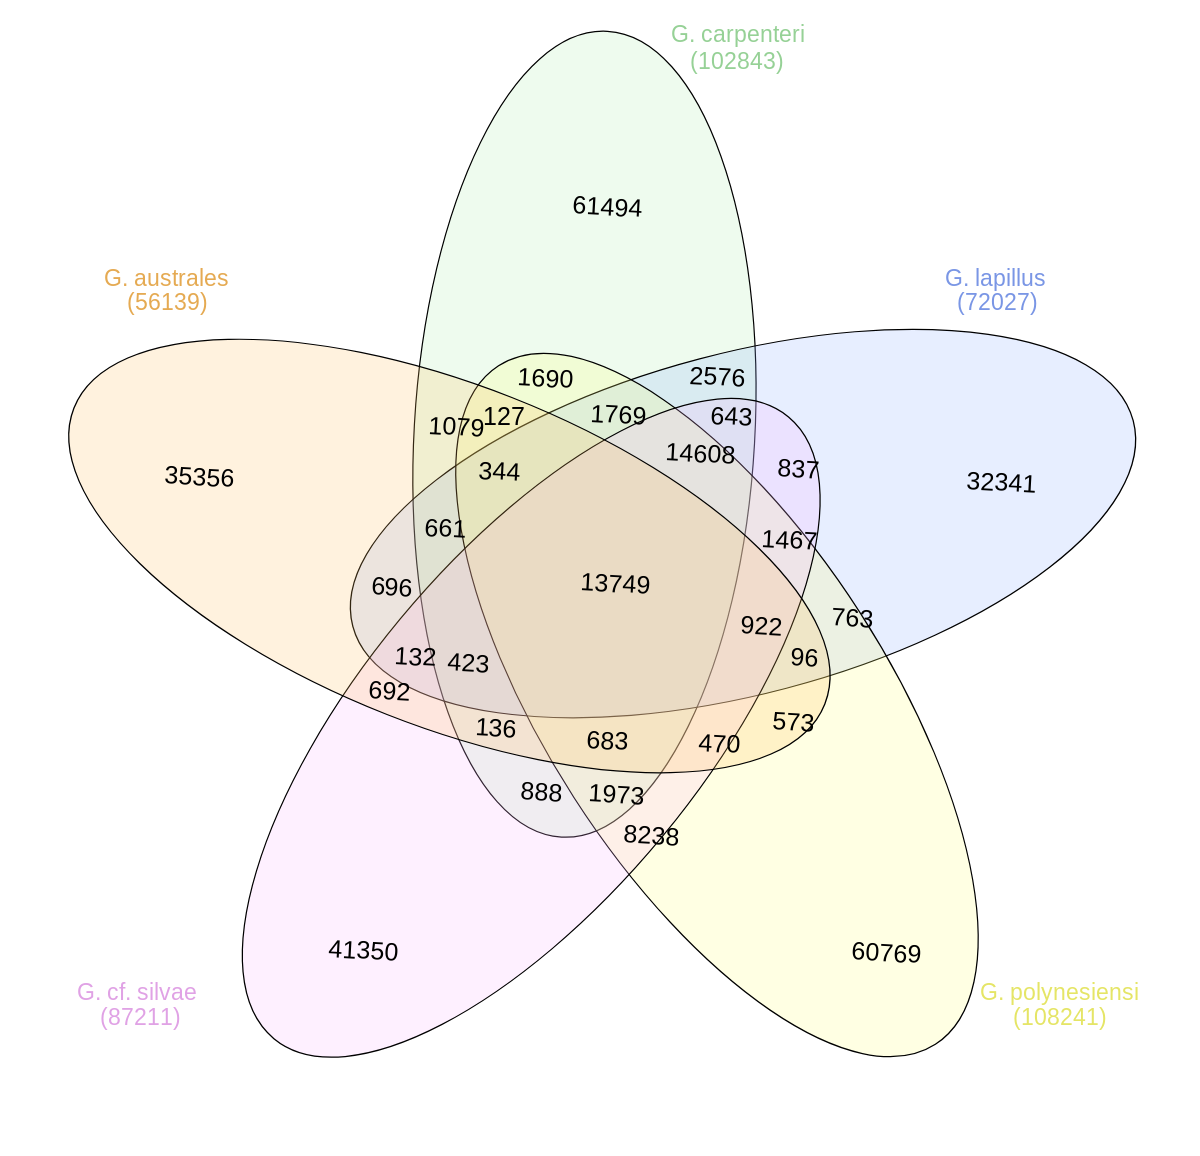
\includegraphics[scale=.4]{3Aug18_cluster-investigation/Species-venn.png} 
\caption{Venn diagram of cluster distribution between the five \textit{Gambierdiscus} species. Core, accessory and inter-species cluster cross over depicted.} 
\label{fig:SpeciesVenn}
\end{figure} 

\begin{table}
\caption{Progression of clusters found in each \emph{Gambierdiscus} transcriptome during processing.}
\label{tbl:ClustTable}
\begin{tabular}{ | p{3cm} | p{2cm} | p{2.5cm} | p{2.5cm} | p{2cm} | p{2cm}|}
\hline
\textbf{Species}& \textit{G. australes}& \emph{G. carpenteri}&\emph{G. lapillus}&\emph{G. polynesiensis}&\emph{G. holmesii}\\
\hline
\textbf{Contigs}&102,863&263,829&148,972&270,315&191,224\\
\hline
\textbf{Spliced leader contigs}&304&683&232&1,570&1,524\\
\hline
\textbf{Nucleotide clusters (cd-hit)}&102,861&263,743&148,966&270,265&191,205\\
\hline
\textbf{Predicted coding regions (Transdecoder)}&63,299&180,568&111,862&176,290&132,688\\
\hline
%\textbf{Protein clusters \# (cd-hit)}&60,166&139,699&92,418&139,487&107,766\\
%\hline
\textbf{Contigs annotated (Interpro Scan)}&131,970&334,737&225,324&225,324&254,844\\ 
\hline
%\textbf{Contigs with Uniprot hits \#}&&&&&\\ 
%\hline
\textbf{Core-transcriptome clusters}&13,750&13,750&13,750&13,750&13,750\\
\hline
\textbf{Softcore-transcriptome clusters}&2,372&16,058&16,297&16,557&16,636\\
\hline
\textbf{Unique clusters}&35,356&61,494&32,341&60,769&41,350\\
\hline
%&&&&&\\
\end{tabular}
\end{table}
\FloatBarrier
\newpage

\subsubsection{Core transcritome}
A set of core genes common to all five species of \textit{Gambierdiscus} were found. 
This set consisted of 13,750 amino acid clusters (Table ~\ref{tbl:ClustTable}) of which 45 \% were annotated with GO terms (Suppl. table ~\ref{tbl:PanGO1} \& ~\ref{tbl:PanGO2}). 
%AD 151218: check grammar in the following sentence - it does not parse
The largest core cluster contained 180 contigs with 
 23, 45, 32, 31 and 49 from \textit{G. australes}, \textit{G. carpenteri} \textit{G. lapillus}, \textit{G. polynesiensis} and \textit{G. holmesii}, respectively, and was of unknown function. 
Twelve of the core clusters contained 100 or more contigs, of which 3 were unannotated. 
The predicted protein coding regions for the other nine clusters, in descending order of contig numbers are: an enzyme with catalytic activity involved in metabolic process, a calcium binding transmembrane transport channel, a protein involved in calcium binding, a protein binding enzyme, a domain for unspecified protein binding, an enzyme with O-glucosyl hydrolase activity involved in carbohydrate metabolic process, membrane bound ion transporter with cation channel activity \& ionotropic glutamate receptor activity, a transmembrane transporter with voltage-gated calcium channel activity, and calcium ion binding transmembrane ion transporter. 
A total of 3,943 core clusters contained 10 or more contigs, meaning that 71.32 \% of the total core clusters consisted of less than 10 contigs. 
The majority of clusters fell within metabolic processes, cellular processes and catalytic activity.% with \%, \% and \% of annotated clusters respectively. 

\subsubsection{Softcore transcriptome}
A soft-core with four out of the five \textit{Gambierdiscus} species examined was identified. 
The soft-core consisted of an additional 16,980 clusters (Table ~\ref{tbl:ClustTable}) of which 48 \% were annotated  (Suppl. table ~\ref{tbl:PanGO1} \& ~\ref{tbl:PanGO2}). 
The most prolific cluster in the soft-core contained 163 contigs with unknown function, where \textit{G. carpenteri} \textit{G. lapillus}, \textit{G. polynesiensis} and \textit{G. holmesii} contained 50, 42, 41 \& 30 contigs respectively. 
A further 5 clusters contained more than 100 contigs, four of which had GO annotations. 
Of the six clusters with over 100 contigs, none had representative contigs from \textit{G. australes}. 
\textit{G. australes} was absent from 86 \% of the softcore clusters. 
In descending order of contigs, they matched to: a protein involved in selective protein binding, a protein involved in actin binding, a protein involved in calcium binding, and a protein with cysteine-type peptidase activity. 
In the soft-core, 14,035 clusters contained 10 or more contigs. 

\subsubsection{Accessory transcriptome}
Clusters with single species representatives, or the accessory transcriptome to the five \textit{Gambierdiscus} species examined, numbered 231,310 clusters. 
Of the unique clusters, only 15.23 \% of clusters were annotated. 
Single species clusters from \emph{G. australes}, \textit{G. carpenteri} \textit{G. lapillus}, \textit{G. polynesiensis} and \textit{G. holmesii} numbered 35,356, 62,494, 32,341, 60,796 \& 41,350 clusters respectively (Table ~\ref{tbl:ClustTable}). 
The highest number of contigs in a unique cluster were 37, found in two clusters from \textit{G. carpenteri}. 
One of these was annotated for RNA and metal ion binding activity. 
Of the unique clusters, 83.1 \% contained only one contig and 97.8 \% of clusters have 5 contigs or less. 

\subsubsection{Comparison of gene ontology annotations.}
\FloatBarrier

The GOs were split up into the three functional groups defined by the consortium: 1) Molecular processes (Figs. ~\ref{fig:SpecGo1Molec}, ~\ref{fig:SpecGo2Molec}, ~\ref{fig:PanGo1Molec} \& ~\ref{fig:PanGo2Molec}) defined as biochemical or a macromolecule directly interacting with other molecules, 2) Cellular components (Figs. ~\ref{fig:SpecGo1Cell}, ~\ref{fig:SpecGo2Cell}, ~\ref{fig:PanGo1Cell} \& ~\ref{fig:PanGo2Cell}) defined by the location within the cell where a molecular process takes place, and 3) Biological process (Figs ~\ref{fig:SpecGo1Bio}, ~\ref{fig:SpecGo2Bio}, ~\ref{fig:PanGo1Bio} \& ~\ref{fig:PanGo2Bio}) which is defined as a molecular machinery participating in the execution of the cell's genetic programming (e.g. cell division).
GO basic is structured in a hierarchical manner, with parent and child terms where parent terms provide a broad overview of functionality and child terms are more specific than parent terms. 
For a general overview of functions present in each transcriptome, level 1 GO terms were elucidated (Figs. ~\ref{fig:SpecGo1Bio}, ~\ref{fig:SpecGo1Cell} ~\ref{fig:SpecGo1Molec}, ~\ref{fig:PanGo1Bio}, ~\ref{fig:PanGo1Cell} \& ~\ref{fig:PanGo1Molec}). 
A more in depth query of the functions present in each transcriptome was conducted with a GO search of the child terms at level 2 (Figs. ~\ref{fig:SpecGo2Bio}, ~\ref{fig:SpecGo2Cell}, ~\ref{fig:SpecGo2Molec}, ~\ref{fig:PanGo2Bio}, ~\ref{fig:PanGo2Cell} \& ~\ref{fig:PanGo2Molec}). 

\paragraph{Level 1 GO annotations between \textit{Gambierdiscus} species.}
\FloatBarrier
The GO annotations found at level 1 between the species of \textit{Gambierdiscus} were similar, with the exception of \textit{G. australes} in several instances. 
GOs assigned part of catalytic activity in molecular processes (Fig. ~\ref{fig:SpecGo1Molec}) as well as both the metabolic and cellular aspects in the biological processes (Fig. ~\ref{fig:SpecGo1Bio}), \textit{G. australes} was underrepresented as compared to the other four species. 
Within the molecular processes (Fig. ~\ref{fig:SpecGo1Molec}), the most common annotation across all five species was for catalytic activity, followed by binding then transporter activities. 
Molecular carrier activity was only registered for \textit{G. australes} and \textit{G. carpenteri} with 1 annotation each.
For GO annotations within the cellular processes (Fig. ~\ref{fig:SpecGo1Cell}), the most common match was to cell parts followed by protein containing complexes then organelle parts. 
\textit{G. carpenteri} and \textit{G. polynesiensis} had one annotation each for cell junction activity. 
The highest number of GOs within biological processes matched to cellular processes (Fig. ~\ref{fig:SpecGo1Bio}), closely followed by metabolic processes then biological regulation and localization. 
The lease represented biological GO annotation was related to growth with only one annotation for \textit{G. holmesii} and \textit{G. polynesiensis}.

\begin{figure} 
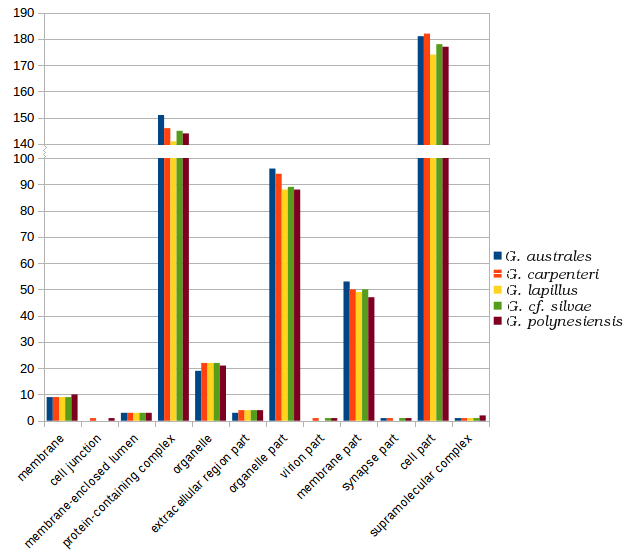
\includegraphics[scale=.9]{3Aug18_cluster-investigation/figures/gosum-species/Species-gosum1-cell-split.png} 
\caption{Summary of cellular GO annotations between \textit{Gambierdiscus} species at GOSUM level 1.}% from Suppl. table ~\ref{tbl:SpGO1}.} 
\label{fig:SpecGo1Cell}
\end{figure} 


\begin{figure} 
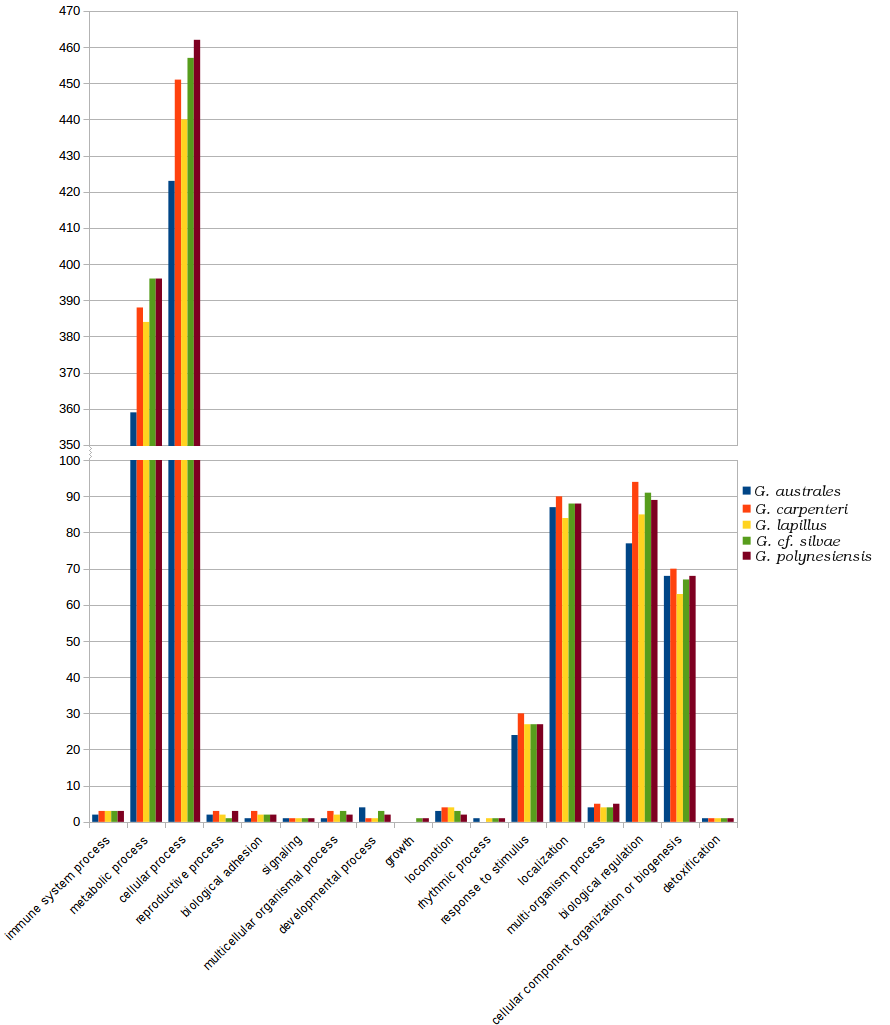
\includegraphics[scale=.7]{3Aug18_cluster-investigation/figures/gosum-species/Species-gosum1-bio-split.png} 
\caption{Summary of biological processes GO annotations between \textit{Gambierdiscus} species at GOSUM level 1.}% from Suppl. table ~\ref{tbl:SpGO1}.} 
\label{fig:SpecGo1Bio}
\end{figure} 



\begin{figure} 
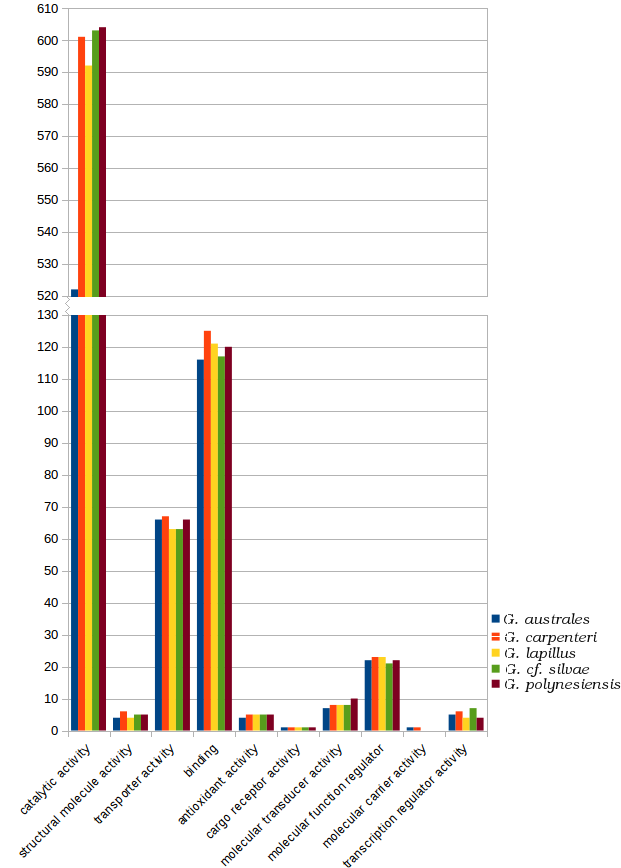
\includegraphics[scale=1]{3Aug18_cluster-investigation/figures/gosum-species/Species-gosum1-molec-split.png} 
\caption{Summary of molecular GO annotations between \textit{Gambierdiscus} species at GOSUM level 1.}% from Suppl. table ~\ref{tbl:SpGO1}.} 
\label{fig:SpecGo1Molec}
\end{figure} 
\FloatBarrier
\paragraph{Level 2 GO annotations between \textit{Gambierdiscus} species.}
\FloatBarrier
At level 2 of GO annotations, the difference between species becomes more apparent. 
While inter-species variations across the molecular, cellular and biological processes (Figs. ~\ref{fig:SpecGo2Bio}, ~\ref{fig:SpecGo2Cell} \& ~\ref{fig:SpecGo2Molec}) are apparent, consistently \textit{G. australes} is underrepresented or absent across all three processes. 
However, \textit{G. australes} was the only species with a small number of GO annotations to nucleocytoplasmic carrier activity as well as general transcription initiation factor activity within the molecular processes. 
Again in the biological processes, \textit{G. australes} was the only species matching to anatomical structure morphogenisis as well as movement within environment as part of symbiotic interaction. 
\textit{G. holmesii} had a much higher representation of GO terms matching sperm-egg recognition. 
The most common molecular processes (Fig. ~\ref{fig:SpecGo2Molec}) mapped to transferase activities, followed by hydrolase activity and oxidoreductase activity. 
For cellular processes (Fig. ~\ref{fig:SpecGo2Cell}) the highest number of GOs was matched to intracellular parts, then intracellular organelle parts and membrane protein complexes. 
Organic substance metabolic processes, cellular metabolic processes and primary metabolic processes had the most GO annotation matches, for the biological processes group ( Fig. ~\ref{fig:SpecGo2Bio}). 

\begin{figure} 
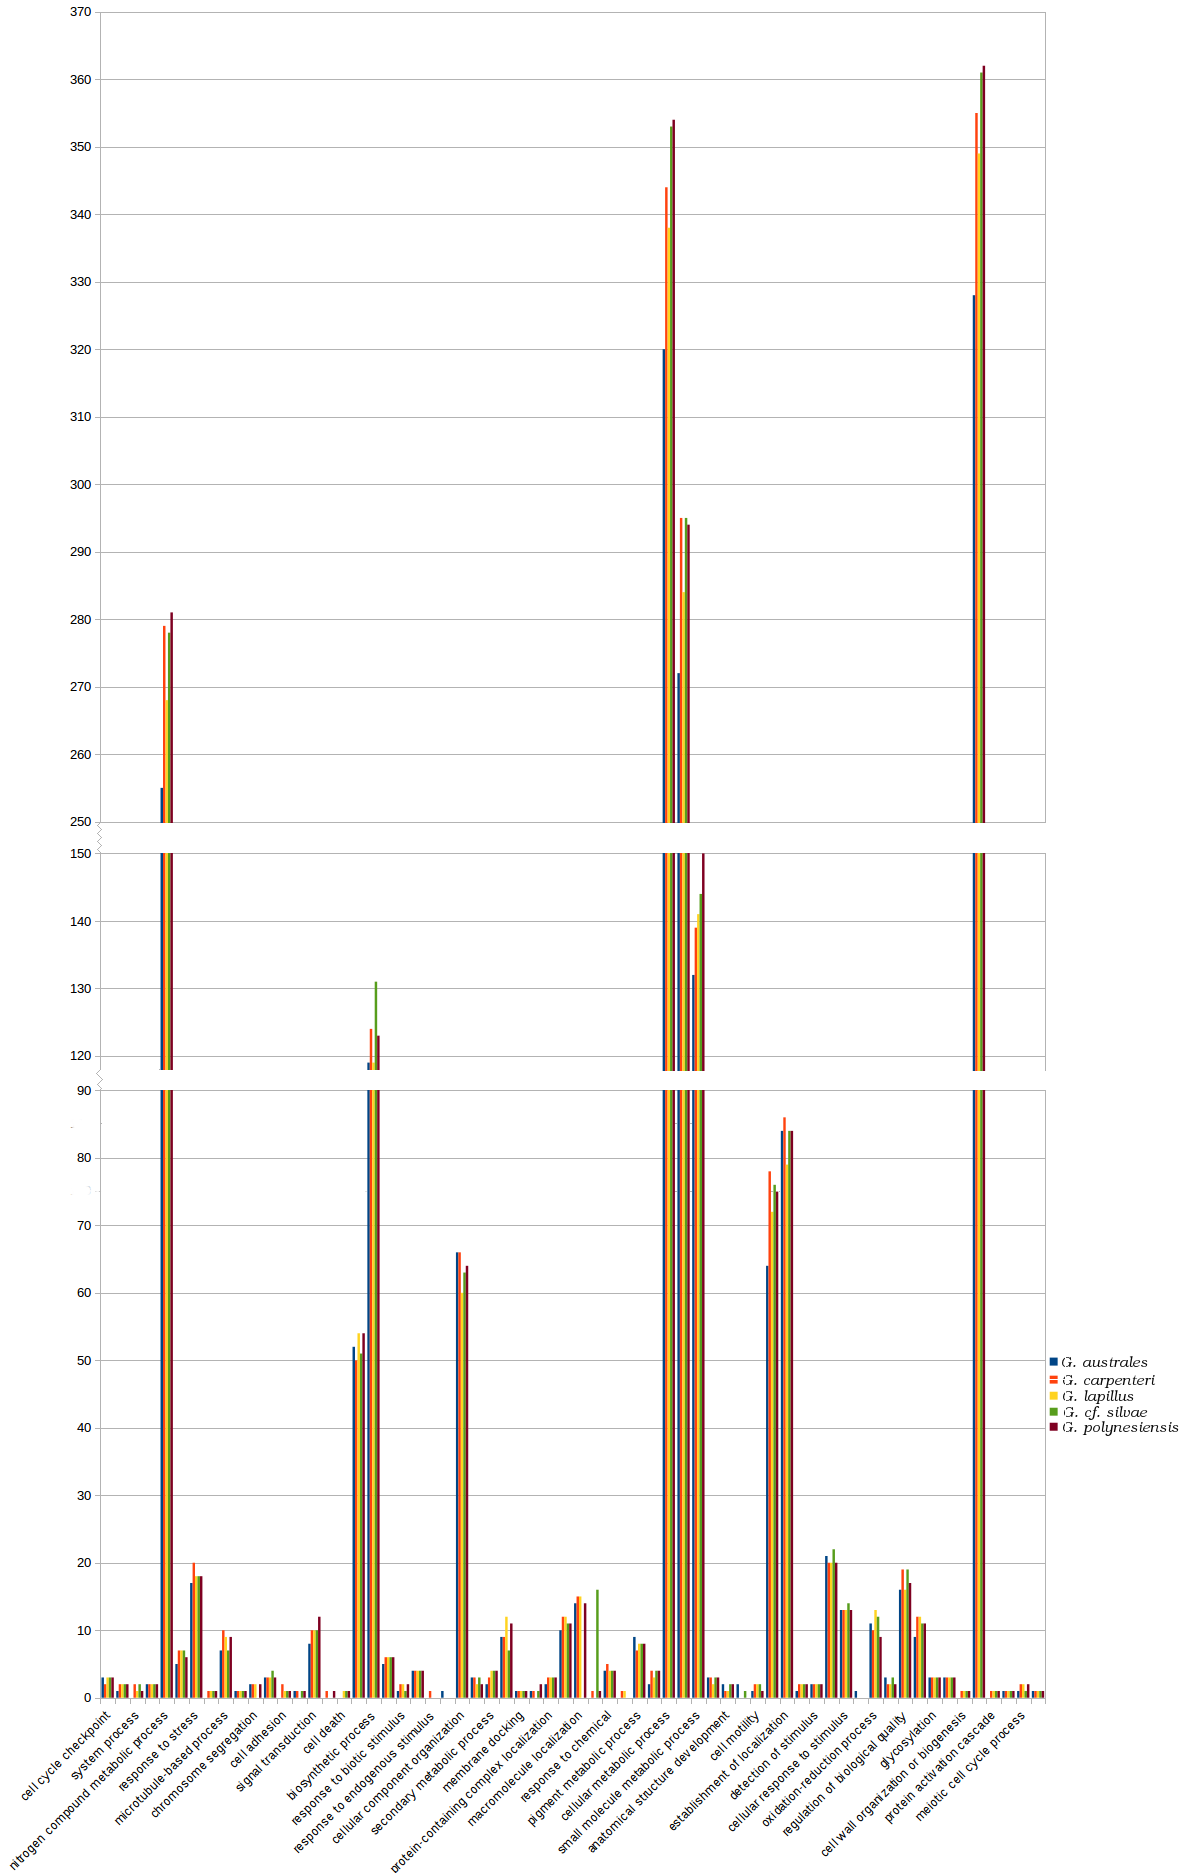
\includegraphics[scale=.45]{3Aug18_cluster-investigation/figures/gosum-species/Species-gosum2-bio2-split.png} 
\caption{Summary of biological processes GO annotations between \textit{Gambierdiscus} species at GOSUM level 2.}% from Suppl. table ~\ref{tbl:SpGO2}.} 
\label{fig:SpecGo2Bio}
\end{figure} 


\begin{figure} 
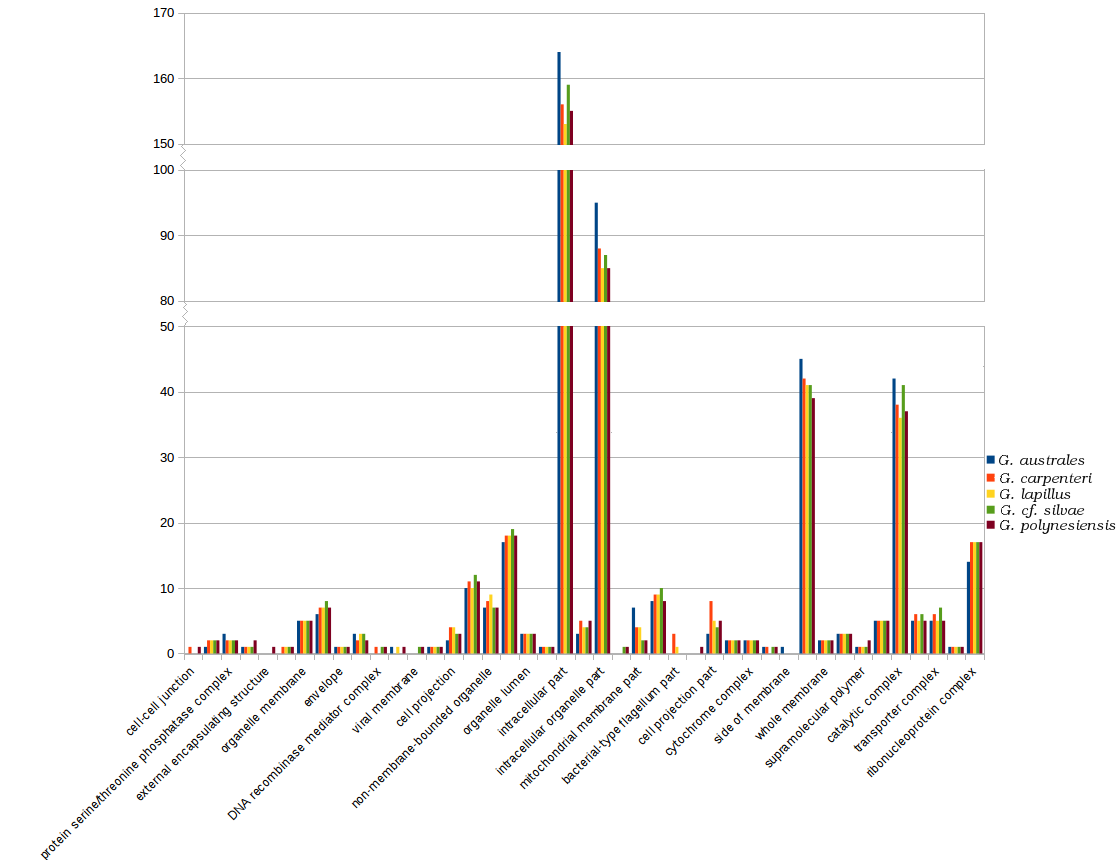
\includegraphics[scale=.6]{3Aug18_cluster-investigation/figures/gosum-species/Species-gosum2-cell2-split.png} 
\caption{Summary of cellular GO annotations between \textit{Gambierdiscus} species at GOSUM level 2.}% from Suppl. table ~\ref{tbl:SpGO2}.} 
\label{fig:SpecGo2Cell}
\end{figure} 


\begin{figure} 
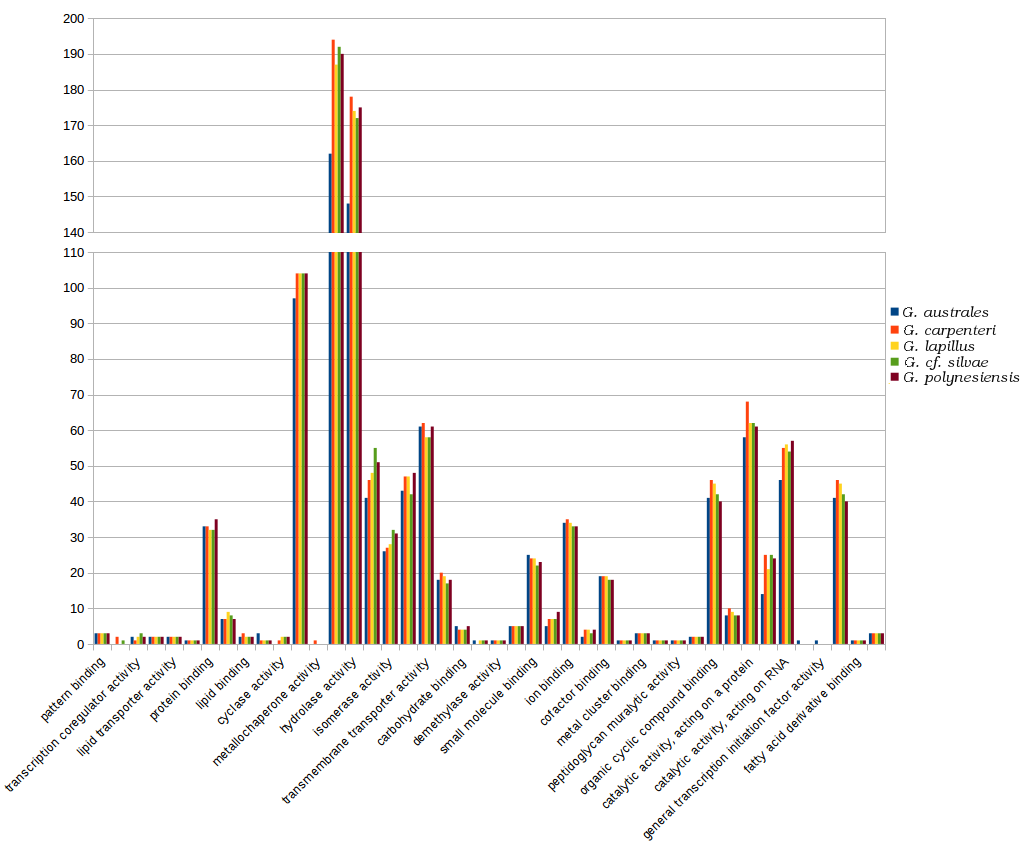
\includegraphics[scale=.6]{3Aug18_cluster-investigation/figures/gosum-species/Species-gosum2-molec-split.png} 
\caption{Summary of molecular GO annotations between \textit{Gambierdiscus} species at GOSUM level 2.}% from Suppl. table ~\ref{tbl:SpGO2}.}  
\label{fig:SpecGo2Molec}
\end{figure} 

\FloatBarrier

\paragraph{Level 1 GO annotations for pan-transcriptomes.}
\FloatBarrier
Similarity between the core, softcore and accessory clusters was consistent across the biological, cellular and molecular processes groups. 
Predominantly the unique clusters had a higher representation in each process with the exception for annotations matching to extracellular region parts and synpase parts within cellular processes (Fig. ~\ref{fig:PanGo1Cell}) as well as developmental processes within the biological processes (Fig. ~\ref{fig:PanGo1Bio}). 
GO annotations most commonly matched to catalytic activity then binding and transporter activities in the molecular processes (Fig. ~\ref{fig:PanGo1Molec}). 
Within the cellular processes, annotations predominantly matched to cellular parts, followed by protein-containing complexes and organelle parts (Fig. ~\ref{fig:PanGo1Bio}). 
For biological processes, the prevalent GO annotations matched to cellular processes, metabolic processes and localization (Fig. ~\ref{fig:PanGo1Bio}).

\begin{figure} 
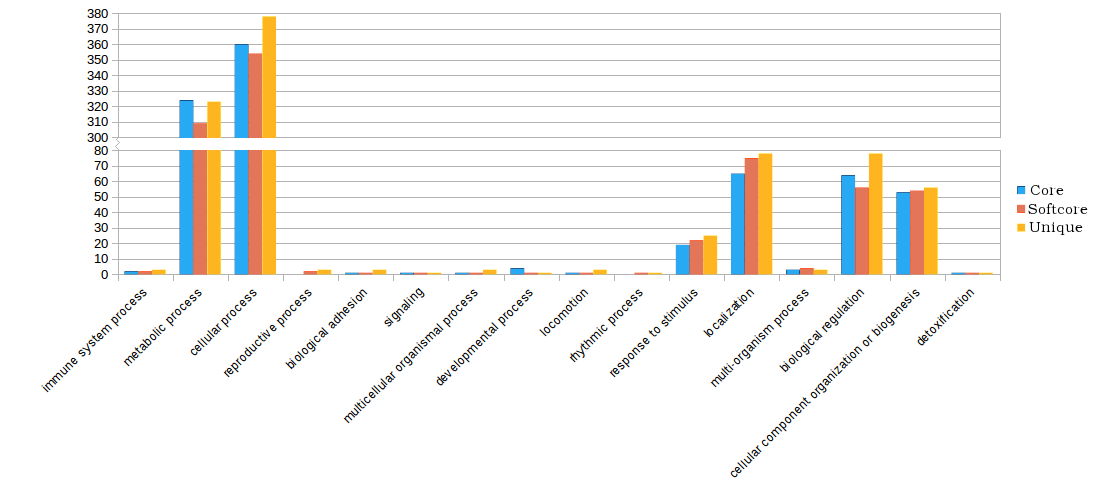
\includegraphics[scale=.58]{3Aug18_cluster-investigation/figures/gosum-pan/Pan-gosum1-bio-split.png} 
\caption{Summary of biological processes GO annotations between core, softcore and unique clusters at GOSUM level 1.} 
\label{fig:PanGo1Bio}
\end{figure} 


\begin{figure} 
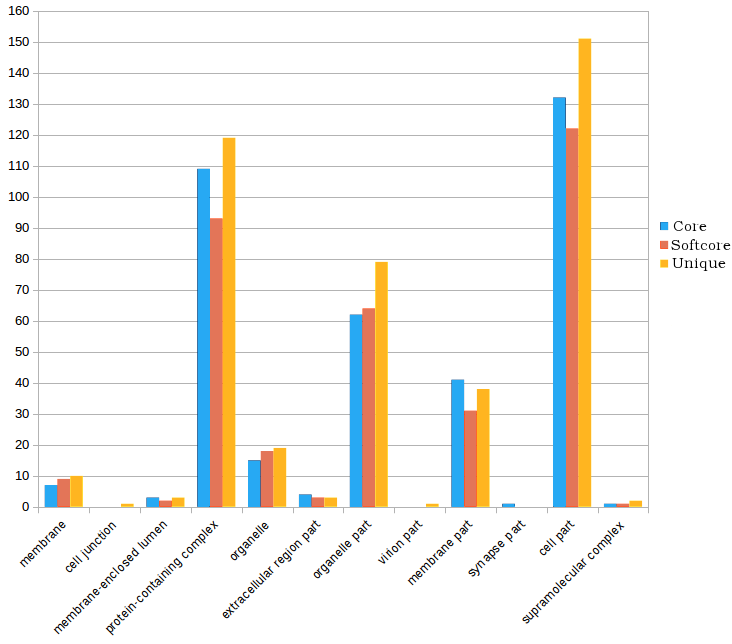
\includegraphics[scale=.8]{3Aug18_cluster-investigation/figures/gosum-pan/Pan-gosum1-cell-split.png} 
\caption{Summary of cellular GO annotations between core, softcore and unique clusters at GOSUM level 1.} 
\label{fig:PanGo1Cell}
\end{figure} 


\begin{figure} 
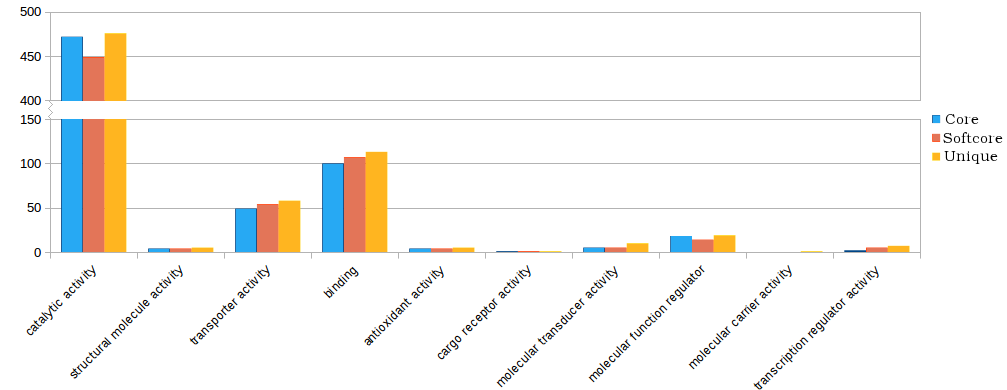
\includegraphics[scale=.6]{3Aug18_cluster-investigation/figures/gosum-pan/Pan-gosum1-molec-split.png} 
\caption{Summary of molecular GO annotations between core, softcore and unique clusters at GOSUM level 1.} 
\label{fig:PanGo1Molec}
\end{figure} 



\FloatBarrier
\paragraph{Level 2 GO annotations for pan-transcriptomes.}
\FloatBarrier
While differences between the biological, cellular and molecular processes were more distinctive at level 2, with the most common pattern among all three groupings of the core and unique clusters closely matching the number of GO terms with one or the other dominant, and the softcore clusters as less prevalent (Figs. ~\ref{fig:PanGo2Bio}, ~\ref{fig:PanGo2Cell} \& ~\ref{fig:PanGo2Molec}). 
Only the unique clusters had annotations matching to DNA binding transcription factor activity, metallochaperone activity and water binding in the molecular processes while the most common GO annotations for the accessory clusters matched to transferase, hydrolase and oxidoreductase activities in descending order (Fig. ~\ref{fig:PanGo2Molec}). 
Within the cellular processes, most annotations matched to intracellular parts, followed by intracellular organelle parts then membrane protein complexes (Fig. ~\ref{fig:PanGo2Cell}). 
Annotations solely from unique clusters were from cell-cell junction complexes, a viral membrane, contractile fibre parts, bacterial-type flagellum and an external encapsulating structure part. 
The biological processes annotations most commonly matched to organic substance metabolic processes, cellular metabolic processes and primary metabolic processes, in descending order (Fig. ~\ref{fig:PanGo2Bio}). 
Unique clusters were the only representatives for system processes, immune response, cell adhesion, cell death, sperm-egg recognition, cell motility and a protein activation cascade. 

\begin{figure} 
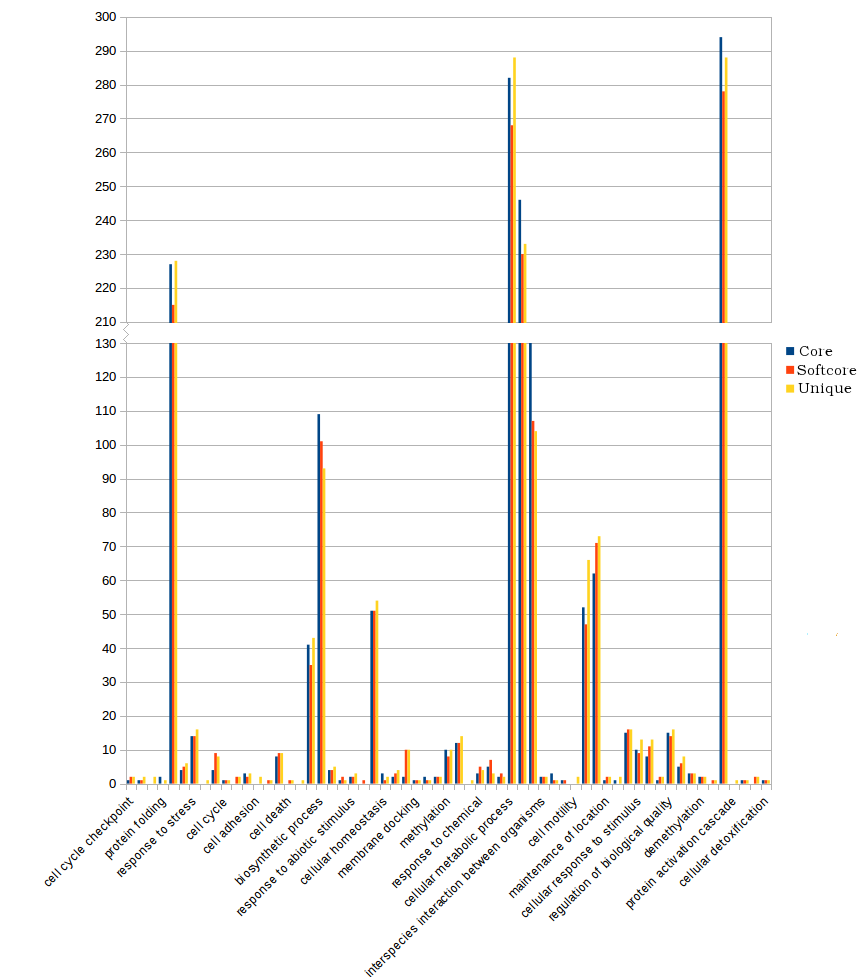
\includegraphics[scale=.75]{3Aug18_cluster-investigation/figures/gosum-pan/Pan-gosum2-bio-split.png} 
\caption{Summary of biological processes GO annotations between core, softcore and unique clusters at GOSUM level 2.} 
\label{fig:PanGo2Bio}
\end{figure} 


\begin{figure} 
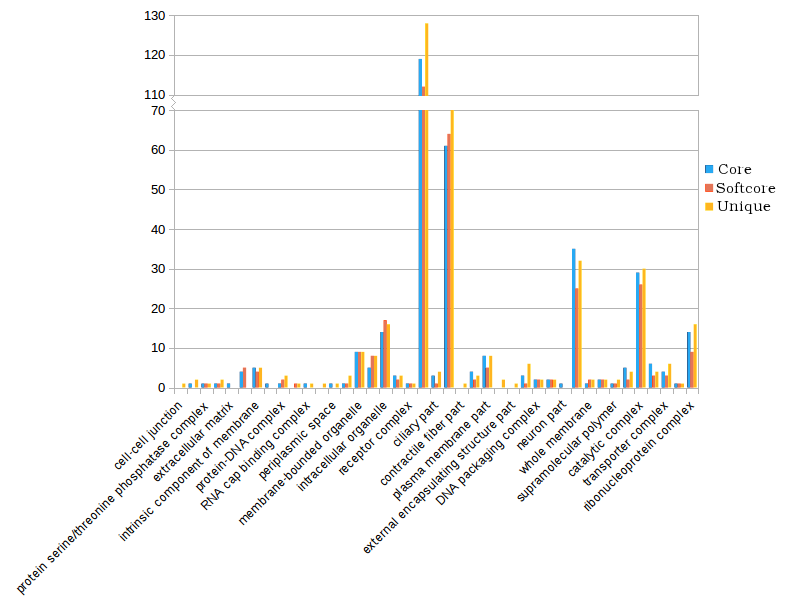
\includegraphics[scale=.8]{3Aug18_cluster-investigation/figures/gosum-pan/Pan-gosum2-cell-split.png} 
\caption{Summary of cellular GO annotations between core, softcore and unique clusters at GOSUM level 2.} 
\label{fig:PanGo2Cell}
\end{figure} 


\begin{figure} 
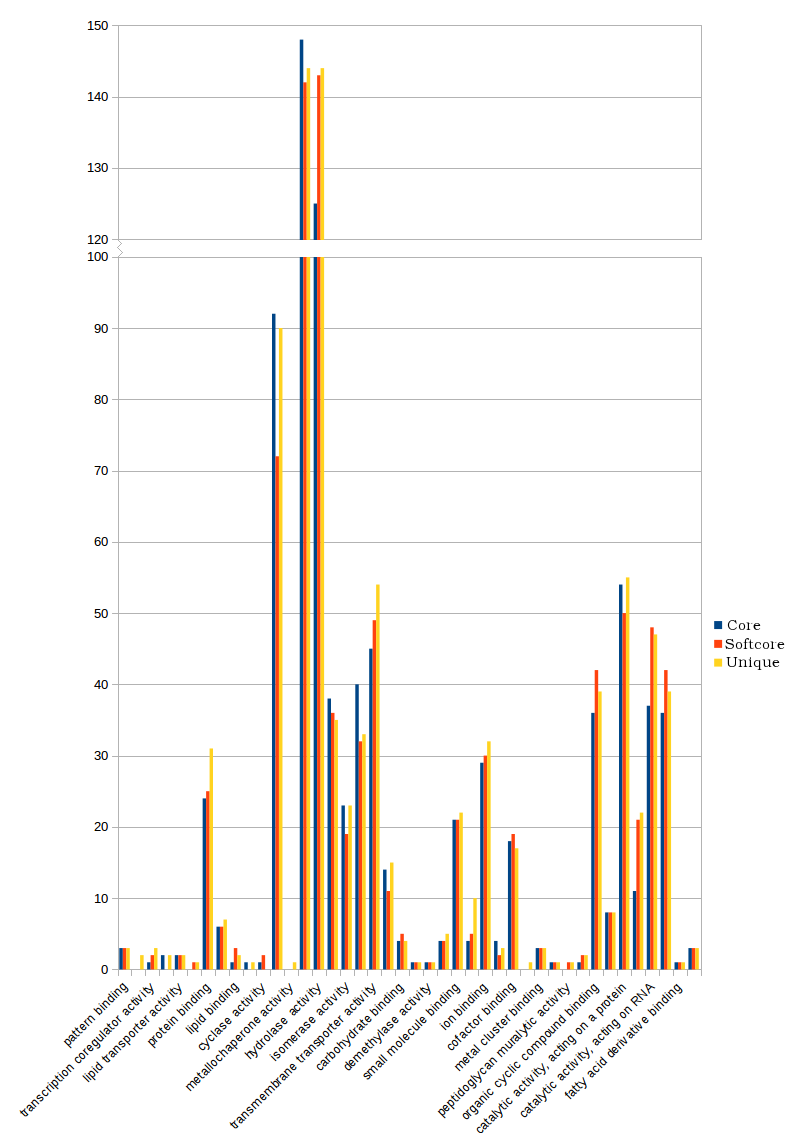
\includegraphics[scale=.78]{3Aug18_cluster-investigation/figures/gosum-pan/Pan-gosum2-molec-split.png} 
\caption{Summary of molecular GO annotations between core, softcore and unique clusters at GOSUM level 2.} 
\label{fig:PanGo2Molec}
\end{figure} 
\FloatBarrier



\subsection{Keto synthase active domain search}
\FloatBarrier
A total of 850 contigs were identified with KS domains which grouped into 314 clusters (Fig. ~\ref{fig:KSVenn}). 
Nine clusters contained more than 10 contigs, with the highest number of 130 contigs from all species.
Nine clusters contained 10 contigs or more, of which only two did not contain all the taxa examined.
Fifty-seven of the 314 clusters contained contigs from multiple species, so 81.8 \% of KS clusters were species specific while 78.7 \% contained only a single contig (Fig. ~\ref{fig:KSVenn}). 
The non-ciguatoxic \textit{G. carpenteri} was absent from 73.6 \% of the clusters. 
Of the clusters without \textit{G. carpenteri}, none contained all four other species. 
However, one cluster contained \textit{G. lapillus}, \textit{G. polynesiensis} and \emph{G. holmesii} with equally represented transcript numbers. 
Four contigs contained \textit{G. polynesiensis} and \emph{G. holmesii} only, one of which had a higher contig representation of \textit{G. polynesiensis} than \emph{G. holmesii}. 
\textit{G. polynesiensis} was the only representative species in 71 clusters, of which three clusters contained 2 contigs and one cluster contained 3 contigs. 
\emph{G. holmesii} was representative as the only species in 23 clusters, one of which contained 3 contigs while the other clusters contained single contigs.
\textit{G. australes}, \textit{G. carpenteri} and \textit{G. lapillus} were the solo representatives of 81, 39 \& 35 KS clusters respectively. \\
\begin{figure} 
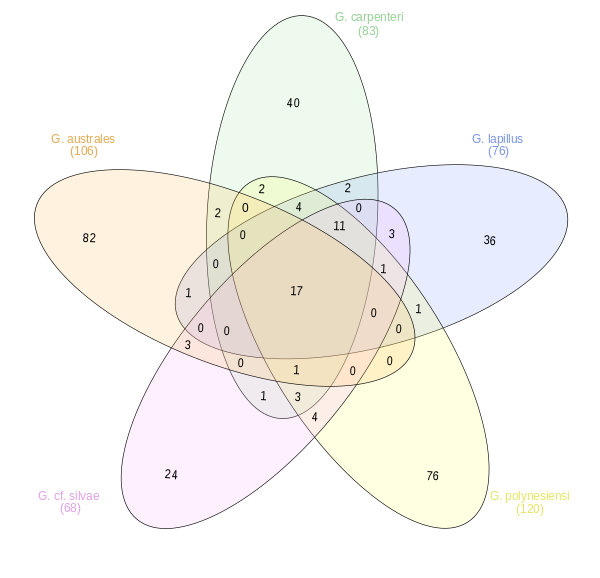
\includegraphics[scale=1]{3Aug18_cluster-investigation/pks/KS-venn.png} 
\caption{Venn diagram of ketosynthase containing clusters distributed across the five \textit{Gambierdiscus} species. Core, accessory and inter-species  ketosynthase cluster cross over depicted.} 
\label{fig:KSVenn}
\end{figure} 
\FloatBarrier

\section{Discussion}
Comparing five \textit{Gambierdiscus} species revealed a core, soft-core and unique fraction in the transcriptomes. 
Further, differences between species with different toxin production characteristics were observed. 
The number of predicted peptides found in this study is high compared to a pan-transcriptome study of four prymnesiophyte algae \cite{koid2014comparative}. 
The predicted peptides in the Koid et al. (2014) study ranged from around 25,000 to 56,000 peptides, where this study found a range from about 63,000 to 270,000 predicted peptides (Table ~\ref{tbl:ClustTable}). 
The lowest number of peptides was predicted in \textit{G. australes}, similar to the findings in the prymnesiophyte algae study and both originating from the MMETSP, where sequencing occurred after a polyA-selection step for isolating eukaryotes \cite{keeling2014marine,koid2014comparative}. 
\textit{G. holmesii} and \textit{G. lapillus} predicted peptides numbered 132,688 and 111,862 respectively, while the highest number of predicted peptides were found in \textit{G. carpenteri} and \textit{G. polynesiensis} at 180,568 and 176,290 respectively. %TODO link ch4 methods
An exploration of the RNA sequencing libraries of two species of \textit{Alexandrium} could not identify common polyadenylation signal sequence motifs \cite{jaeckisch2011comparative}. 
The implication is that the polyadenylation signal is removed during mRNA processing, in at least some dinoflagellates \cite{bachvaroff2008stop,jaeckisch2011comparative}. 
As the MMETSP transcriptomes had been sequenced after polyadenylation selection of transcripts, the comparatively low numbers of predicted peptides for \textit{G. australes} as well as the prymnesiophyte algae could be accounted for by the loss of eukaryotic mRNA that had been processed to remove the polyadenylation signal.\\
The abundance of dinoSL was quite low (Table ~\ref{tbl:ClustTable}) compared to the abundance observed by Zhang et al. (2009) in \textit{Amphidinium carterae}. 
Similar to this study, a low abundance of spliced leaders has been observed in other dinoflagellates \cite{guo2011spliced,bachvaroff2008stop}. 
The function of the spliced leader, and hence whether this variation in observation between high and low abundance is species specific or due to assembly method employed, is as yet unknown.
Interestingly, \textit{G. holmesii} and \textit{G. polynesiensis} had the most contigs with dinoSLs. 
These were sequenced with different read lengths and collected from different geographic locations, but are phylogenetically in the same \textit{Gambierdiscus} sub-clade. %TODO link appendix holmesii paper

\subsection{Core, softcore and accessory genes}
The number of contigs and predicted peptides from this study was markedly less for \textit{G. australes}, from the MMETSP dataset, in comparison to the transcriptome assemblies generated in \textbf{Chapter 4}. 
To accommodate for the low number of contigs from \textit{G. australes}, the softcore spanned 4 of the 5 taxa. 
Noticeably, \textit{G. australes} was absent from 86 \% of the softcore dataset which indicates that a large proportion of the softcore is likely part of the \textit{Gambierdiscus} pan-transcriptome core which was not captured in the \textit{G. australes} sequencing. 
This is an example highlighting the value of a reference pan-transcriptome.\\
There was no distinct difference between the species GO annotations, with the exception of \textit{G. australes}. 
This is as expected, as the species operate under similar nutritional modes and within similar temperature ranges \cite{kibler2012growth,parsons2012gambierdiscus} and were isolated from tropical or sub-tropical conditions, apart from \textit{G. carpenteri} which was isolated from the temperate Merimbula region \cite{larsson2018toxicology}. \\
No difference was observed in the biological, cellular and molecular GO annotation groups at levels 1 and 2 between the core, softcore and accessory clusters. 
This is somewhat less expected as as it would be reasonable to predict a functional difference for genes unique to each species. 
Possible reasons could be that this observation only captures predicted peptides with GO annotations which were only 15.23 \% of the 231,310 accessory clusters. 
This indicates that no functional match for over 196,000 of the accessory clusters could be found and no indication what their function might be could be extrapolated. 
As dinoflagellate sequencing and genome exploration is still comparably sparse, it follows that a lack of annotated references in the sequencing databases translates to low annotation rates.
The need for annotations and a comparable reference transcriptome becomes apparent when investigating genetic elements as uncharacterized as these.

\subsection{Ketosynthase domain detection}
Between all five species, 850 contigs with KS domains were identified. 
These resolved into 314 clusters, of which 17 were shared among all species. 
The majority (81.8 \%) resolved as unique clusters per species, ranging from 24 clusters for \textit{G. holmesii} to 82 clusters for \textit{G. australes}. 
The toxin profile for \textit{G. polynesiensis} and the toxicity assay conducted by Larsson et al. (2018) for \textit{G. holmesii} indicate that these two species are the most ciguatoxic of the taxa included in this study. 
While \textit{G. lapillus} displayed lower levels of ciguatoxicity in bioassays, the strain included here (HG4) was the least toxic of the \textit{G. lapillus} strains tested in \textbf{Chapter 2}. %TODO link ch2 toxicity section 
Four KS clusters included \textit{G. holmesii} and \textit{G. polynesiensis} only, one of which contained 4 contigs from \textit{G. polynesiensis} and 1 from \textit{G. holmesii}. 
A further 22 and 75 clusters only contained \textit{G. holmesii} and \textit{G. polynesiensis} contigs respectively. 
These clusters                                                                                                                                                                                                                                                                                                                                                                                                                                                                                                                                                                                                                                                                                                                                                                                                                                                                 could be of interest for further investigation into KS domains involved in CTX synthesis. 


\subsection{Areas for possible improvement in this study}
This chapter presents a novel approach to analyzing \textit{Gambierdiscus} transcriptomes and possible avenues for investigation for ciguatoxin production pathways. 
However, there are several aspects that can be improved upon with future studies.

\paragraph{Contaminants in dataset.}
The RNA-seq libraries were constructed from whole RNA seq runs with non-axenic cultures, hence it is likely that bacterial RNA is a subset of the analysis. 
It is unlikely that the same contamination persists in the core and softcore clusters, i.e. across all four to five species collected from Australia, the Cook Islands and over a 10 year time span. 
However the unique clusters could well be contaminated with non-eukaryotic contigs, which is indicated by some of the unique clusters only annotations mapping to a bacterial flagellum and a viral capsid. %TODO link to results section 
Hence it would be pertinent to  devise a method to separate bacterial from eukaryotic contigs post sequencing. 


\paragraph{Coverage of taxa.}
As with bacterial pan-transcriptomics, eukaryotic studies reveal a correlation between the number of species and strains included for refining the core transcriptome and expanding the unique fraction of the transcriptome \cite{koid2014comparative,tettelin2005genome,jin2016maize}. 
For \textit{Gambierdiscus}, including several strains of a species is essential for the discovery of a non-ciguatoxic \textit{G. polynesiensis} strain \cite{rhodes2017epiphytic}. 
Variability in morphology and toxicity has also been observed in \textit{G. lapillus} \cite{kretzschmar2017characterization}. 
While this study sought to cover taxa from the three main \textit{Gambierdiscus} clades, an increase in species and strain coverage is highly likely to impact the resolution of the core and unique portions especially as the sequencing coverage of the \textit{G. australes} transcriptome is less in depth than the other four species (Table ~\ref{tbl:ClustTable}).
Hence due to limited species and the singular strain per species coverage, this represents an exploratory study for establishing a pan-transcriptome for \textit{Gambierdiscus} which should be improved upon. 

\paragraph{PKS active domain search.}
PKS complexes consist of a number of active domains that synthesize and manipulate the polyketide backbone. 
The KS domain is but one of several essential domains for a functional polyketide. 
The search for active domains should be extended to include other domains for comparison in the search for the ciguatoxin production pathways.

%\newpage
\section*{Conclusion}
Protists represent a large section of the tree of life and are involved in vital geochemical cycling, symbiotic and toxic relationships in their environment. 
Yet due to the convoluted nature of their genomes, querying the genetic content of these organisms is fraught with obstacles. 
This study presents a pan-transcriptome for the genus \textit{Gambierdiscus}, some species of which are involved in CTX production. 
The approach opens up an alternative avenue for investigation of the differences and similarities of toxic \textit{Gambierdiscus} species in general, and specifically in regard to the toxin production pathway(s). 
This study provides a starting point for \textit{Gambierdiscus} pan-transcriptomic exploration and a rudimentary reference for future sequencing efforts.
It is recommended that this dataset is expanded to encompass both more \textit{Gambierdiscus} species and strains to crystallize the genus' pan-transcriptome in more detail.


\clearpage% Flush page

\newpage
\bibliographystyle{acm}
\bibliography{pantran.bib}


\end{document}
